\documentclass[a4paper,twoside]{article}

\usepackage{epsfig}
\usepackage{subcaption}
\usepackage{calc}
\usepackage{comment}
\usepackage{amssymb}
\usepackage{amstext}
\usepackage{amsmath}
\usepackage{amsthm}
\usepackage{multicol}
\usepackage{pslatex}
\usepackage{apalike}
\usepackage{xcolor}
\usepackage{multirow}
\usepackage{array}
\usepackage{SCITEPRESS}
\usepackage{graphicx} % Please add other packages that you may need BEFORE the SCITEPRESS.sty package.

\newcommand{\head}[1]{\textbf{#1}}
\newcolumntype{C}[1]{>{\centering\arraybackslash}p{#1}}


\begin{document}

\title{A Case Study on Performance Optimization Techniques in Java Programming}

\author{\authorname{Ciprian Khlud\sup{1}\orcidAuthor{0000-0001-6211-3199}
  and Cristian Fr\u asinaru\sup{1}\orcidAuthor{0000-0002-5246-7396} }
\affiliation{\sup{1}"Alexandru Ioan Cuza University", Ia\c si, Romania}
\email{ciprian.mustiata@gmail.com, acf@info.uaic.ro}
}

\keywords{Java, Runtime performance, Memory usage, Garbage collection, Sequence analysis, SAM/BAM files}

\abstract{
Choosing the right programming platform for processor or memory intensive applications is a subject that is debated in all types of contexts.
When analyzing the performance of a specific platform, equally important is the usage of appropriate language specific constructions and 
programming interfaces (APIs).
In this paper we investigate how a state-of-the art implementation, part of a multi-threaded framework for sequence analysis (elPrep)
could benefit from various optimization techniques dedicated to improving the runtime performance of Java applications.
ElPrep is an established tool for processing SAM and BAM files in sequencing pipelines. 
In order to migrate from its original implementation to a different software platform, more suitable for memory intensive tasks, 
the authors have re-implemented elPrep in Java, Go and C++ and benchmarked their performance.
Overall, the Go implementation won by a good margin, considering a metric that involved both the RAM usage and the runtime performance.
We show that, without changing the semantics of the algorithm, by using appropriate programming techniques we are able to significantly improve the behavior of the Java implementation to a point that may even alter the conclusions of the original study. 
We also show that, by changing the manner in which data is represented, to better fit the particulars of the Java memory management, we are able to improve the original scoring (based on computing time and memory consumption) to around one order of magnitude better on the most expensive component (read/write).
}
%We also show that with changing the semantics of the algorithm, especially focusing on memory consumption, we are able to improve the original scoring (based of a composite of compute time and memory) to around one order of magnitude better on the most expensive component (read/write).

\onecolumn \maketitle \normalsize \setcounter{footnote}{0} \vfill

\section{\uppercase{Introduction}}
\label{sec:introduction}

In the field of bioinformatics, DNA sequence analysis generally consists of processing large amounts of data and performing various operations on it, 
such as sequence alignment, variant detection, searches against biological databases, etc.
A large variety of software tools exists for these operations, most of them having specific uses cases but with a common denominator 
regarding the fact they need to perform processor and memory intensive tasks: 
I/O operations on large file, compression/decompression, text processing, etc.~\cite{?}

Choosing a programming platform that offers all the required instruments to handle the specific challenges in bioinformatics is important, 
as pointed out in a recent study dedicated to migrating an existing Common Lisp application, called elPrep, 
to another platform with better support for memory management and concurrency~\cite{costanza:2019}.
ElPrep~\cite{herzeel:2019} is a a multithreaded tool for preparing sequence alignment/map files (SAM/BAM)
for variant calling in DNA sequencing pipelines. 
A key feature of elPrep is the ability to avoid the standard practice of creating a pipeline consisting of multiple command line tools invocations, 
executing a single pass through a SAM/BAM file and keeping data as much as possible in main memory.
%As the software executes concurrently different steps of the algorithm, it needs to process large amounts of data (hundreds of gigabytes) in an efficient way.
In~\cite{costanza:2019} the authors investigated Go, Java and C++ programming platforms, as an alternative to Common Lisp.
%Go and Java using a concurrent, parallel garbage collector on the one hand, and C++17 using reference counting on the other hand for handling
Te result of their study concluded that the Go implementation performed best, using a metric that involved both the RAM usage and the runtime performance.
The benchmarks of the study showed that Java had a faster runtime, but a significantly higher memory usage, while Go offered a better balance between the two.

As the Java source code for elPrep is available at {\texttt{https://github.com/exascience/elprep-bench} }, we have analyzed key aspects regarding the memory management and
thread synchronization, and propose a series of improvements that could increase significantly the performance of the Java implementation. 
%benefit other studies of this kind.


\section{\uppercase{Background}}\label{sec:uppercase5}

\subsection{\uppercase{Garbage Collection}}\label{subsec:uppercase14}

In order to analyze the behavior of memory intensive applications,
%especially those based on frequent allocation and deallocation, 
it is important to understand how garbage collection works and especially how Java~\cite{java} implements its garbage collectors.

The Java Virtual Machine (JVM)~\cite{lindholm:2014} offers an automatic storage management system, called {\textit{garbage collector}  (GC)} which reclaims heap storage occupied by objects which are no longer used.
The garbage collection process~\cite{gc:oracle} works typically by splitting the heap into two regions: a {\textit{young generation} } region and an {\textit{old generation} }.
All new objects are allocated in the young region, in a very fast manner, using typically a "bump-pointer" strategy.
When this region becomes full  a {\textit{minor} } garbage collection occurs and all dead objects are deleted very quickly.
The objects which are still referenced survive and they  are moved to the old generation.
This minor collection is always a "stop the world" event, meaning that all of the application threads will be paused until the GC is finished.
In the old generation, objects are expected to live longer and they are collected more seldom but with a more expensive algorithm, called {\textit{major} } garbage collection.

The algorithm used by GC has two steps.
The first one is to {\textit{mark} } the objects that are still used from the heap.
In the second step, it {\textit{sweeps}  (deletes)} the objects which have not been marked (dead), leaving only referenced objects and pointers to free space.
%To further improve performance, in addition to deleting unreferenced objects, you can also compact the remaining referenced objects.
By moving referenced object together, this makes new memory allocation much easier and faster.
Therefore, the speed of GC depends on two factors: the number of objects it has to analyze and the complexity of the relationships between them. %collecting graph

Considering the behavior we have described so far, we will analyze the impact of some simple tweaks
meant to reduce the impact of GC over the application performance, such as:
reducing the unnecessary small allocations in young region, controlling the scope in which objects are referenced in order to minimize the number of times when expensive collection of old region is triggered, simplifying the object graph and controlling the amount of memory JVM is allowed to use.


\subsection{\uppercase{Threads, Locks and the File System}}\label{subsec:uppercase13}

Java platform supports concurrent programming by using threads~\cite{gosling:2014}.
Multiple threads can execute at the same time, taking advantage of computing units that have more than one processor and of processors that have more than one core.
Threads performing operations that are not atomic will interleave when they access shared data.
A {\textit{synchronized} } statement acquires a mutual-exclusion lock when entering a critical section, executes the block that references the shared data, then releases the lock.
While one thread owns the lock for that data, no other thread may access it. 
The proper use of this mechanism is crucial for the concurrent implementation of an algorithm.
If threads are waiting to much on locked resources, the overall performance of the application will suffer.

In our case study, multiple threads are performing operations on the file system, reading and writing large amounts of strings from and into text files.
Regardless of the operating system and programming language, the underlying hardware is optimized to work with streams of bytes.
In an atomic operation, data is read into a buffer of bytes, in a contiguous manner.
Similarly, data is written into a buffer of bytes that is flushed afterwards to the file.
Both these operations are single threaded by design and historical reasons, so Java libraries have locks to make the access to streams single-threaded.
A \texttt{write} method usually looks like this:
\begin{small}
\begin{verbatim}
public void write(String s, int off, int len){
  synchronized (lock) { ... }
}
\end{verbatim}
\end{small}

%The algorithm for writing to disk is the following:
%
%\begin{small}
%	\begin{verbatim}
%	allSamAlignments.map(
%	  samAlignment -> formatRow(samAlignment);
%	)
%	.forEach(
%	  formattedRow -> writeToBuffer(formattedRow));
%	\end{verbatim}
%\end{small}

We will show that creating a large number of short lived strings and writing them to a file in a multithreaded manner will generate a behavior similar to using a single thread, plus the overhead of acquiring and releasing the synchronization lock.


%So what we did, we rewrote the code to be single threaded, so we don't call any OS to lock and release a mutex and the pseudo-code would look like following:
%
%\begin{small}
%	\begin{verbatim}
%allSamAlignments.forEach(samAlignment ->
%{
%  writeToBufferFormatted(samAlignment);
%});
%	\end{verbatim}
%\end{small}

%The main take away is that the updated code can write directly to underlying buffer and it can be made quite fast and it will need basically no allocation, as it will be shown.


\subsection{\uppercase{Memory Usage}}\label{subsec:uppercase12}

The Java Virtual Machine allocates memory either on stack or on heap~\cite{lindholm:2014}.

The {\textit{heap} } is the place where all class instances and arrays are allocated and it is shared among all threads.
Each JVM thread has a private {\textit{stack} } which holds local variables and partial results  during successive method invocations and returns.
%The JVM might do escape analysis and decide to allocate objects directly on the stack, which means cleaning them up when the method ends is free.
When working with large amounts of objects, it is quite important to assess the memory consumption of a data structure, in similar way as the {\textit{sizeof} } construct in C or C++.
%JVMs may move some heap allocations to stack allocations, but this would not matter if we allocate long running objects and as we talked in section about GC, the GC will have also some pre-allocated memory to do future expected allocations.
An object allocated on the heap has a {\textit{header} } which contains information used for locking, garbage collection or the identity of that object.
The size of the header depends on the operating system, and it may be 8 bytes on 32 bit architectures or 16 bytes on 64 bit architectures.
Also, for performance reasons and in order to conform with most of the hardware architectures, JVM will {\textit{align} } data.
That means that if we have an object that wraps just one byte, it will not use: $8 \text{(object header)} + 1 \text{(content)} = 9 $ bytes of memory on the heap, but it will use $16$ bytes as it needs to be aligned to the next $8$ byte boundary.
%A technical brief description made by a JVM engineer describes why and how was it done: https://shipilev.net/jvm/anatomy-quarks/24-object-alignment/

In Java, strings are objects and they are allocated on the heap.
That fact that string literals are stored in a shared object pool, in order to reduce memory consumption, is of no relevance in our context.
Inspecting the source code of the \texttt{String} class, one can observe the following instance fields:
\begin{small}
\begin{verbatim}
private final byte[] value;
private final byte coder;
private int hash;
// Defaults to 0
\end{verbatim}
\end{small}

As expected, a \texttt{String} object keeps a reference to an internal byte array.
However, the other two fields will make the size of the object equal to: $8$ (header) $+$ $4$ \texttt{value} reference $+$ $1$  \texttt{coder} value $+$ $4$ \texttt{hash} value $= 17$ bytes.
Being aligned to $8$ bytes, it will actually use $24$ bytes.
When creating many \texttt{String} instances (like millions of them, as in our case study), the extra information included in this class will add up, consuming memory and  triggering the garbage collector more often than necessary. 

We will show that replacing the \texttt{String} usage to the underlying \texttt{value} byte array will improve the performance of the application, and this approach should be implemented in every scenario that involves processing large amounts of text data.
% especially if it is done at million times scale, will be translated both in fewer GCs (as are saved few tenths of MB), fewer 24 bytes * million instances bytes to copy and visit for marking. 



\subsection{\uppercase{Memory Compaction}}\label{subsec:uppercase}
Another important part of working with large data sets that have to be accessible in memory regards the format in which they are represented.
Choosing the right format will not only reduce the amount of consumed memory but it will also reduce the GC cost to copy the objects between regions and the cost of visiting and marking them.

The most common approach of representing information is in row based form, where a {\textit{row} } is a record of some kind and a {\textit{column} } is a certain property of that row.
This type of representation is used in most relational databases management systems, where sets of rows of the same type form {\textit{tables} }.
Despite having many advantages, this format is not necessarily optimum when it comes to data representation in memory.

A {\textit{column store} } model~\cite{abadi:2013} "reverses" the orientation of the tables.
It stores data by columns and uses row identifiers in order to access a specific cell of the table.
By storing each column separately, query performance is increased in certain contexts as they are able to read only the required attributes, rather than having to read entire rows from disk and discard unneeded attributes once they are in memory.
Another benefit is that column stores are very efficient at data compression, since representing information of the same type inside of a column helps the {\textit{data alignment} } process that we have previously mentioned.

Let's consider a simple example, using the class {\texttt{Point} }, defined as a pair of two integer fields {\texttt{x} } and {\texttt{y} }.
The basic idea is that instead of having a row-based model consisting of an array {\texttt{Point} []} of instances (each {\texttt{Point} } object is a row and its members {\texttt{x} } and {\texttt{y} } are the columns), to use two arrays of integers {\texttt{x} []} and {\texttt{y} []}, representing the two columns.
%and one integer index for each {\tt Point}.
This way we can store the same data, minus the object headers corresponding to all the {\texttt{Point} } instances.
Not only the memory consumption will be lower (so the GC will be triggered less often), but the structure will also take shorter time to visit, since there are only two objects now (the two arrays).

Though a column store is a very good solution for size reduction, it has the downside of requiring more computational effort in order to work with multiple properties of the same object.
However, when saving memory is the major concern, and especially when it comes to hundreds of GB per instance, the execution slowdown becomes far less important if we can achieve significant reductions in consumed memory.



\section{\uppercase{Representing the Data Store}}\label{sec:uppercase4}

\subsection{\uppercase{The Row-Based Model}}\label{subsec:uppercase11}

The data structure which is used in original ElPrep algorithm is represented by the class {\texttt{SamAlignment} }, an object of this type storing one row of a SAM file.
The class contains the following declaration of instance variables:

\begin{small}
\begin{verbatim}
public Slice QNAME;
public char FLAG;
public Slice RNAME;
public int POS;
public byte MAPQ;
public Slice CIGAR;
public Slice RNEXT;
public int PNEXT;
public int TLEN;
public Slice SEQ;
public Slice QUAL;
public List<Field> TAGS = new ArrayList<>(16);
public List<Field> temps = new ArrayList<>(4);
\end{verbatim}
\end{small}

For a small BAM file of 144 MB there will be created around $2.1$ million {\texttt{SamAlignment} } instances and for a $1.27$ GB BAM file there will be created around $17.6$ million objects.

For simplicity, let's disregard {\texttt{TAGS} } and {\texttt{temps} } fields (which can have different lengths) as it makes the calculation simpler and analyze the memory consumption in both cases.
We suppose also that the JVM uses 32 bits for representing an object header.

One {\texttt{SamAlignment} } object contains:
8 bytes object header, 6 instances of {\texttt{Slice} } objects ({\texttt{QNAME} }, {\texttt{RNAME} }, {\texttt{CIGAR} }, {\texttt{RNEXT} }, {\texttt{SEQ} }, {\texttt{QUAL} }) of 4 bytes each, 3 integer fields ({\texttt{POS} }, {\texttt{PNEXT} }, {\texttt{TLEN} }) of 4 bytes each, 1 character ({\texttt{FLAG} }) of 2 bytes, and an additional byte ({\texttt{MAPQ} }).
So, the total size of the object is: $8 + 6 * 4 + 3*4  + 1 * 2+ 1 * 1 = 47$ bytes, and as it is rounded up to a multiple of $8$, the result is $48$ bytes.
%For a 64 bit JVM without compressed OPS, the comsumption is of only SAMAlignment instances is: 12 + 6*8+3*4+1*2+1*1 = 75 and as it is 8 bytes rounded up, the consumption is 80 bytes

In order to save memory, the string representing a row scanned from the original file is shared between multiple objects.
All $6$ {\texttt{Slice} } instances contain a reference to the  underlying string and two integers pointing to the start index and length.
So, a {\texttt{Slice} } instance uses: $8$ (object header) $+4$ (reference to the string) $ + 4 + 4 = 20$ bytes, being rounded to $24$.

%For 64 bit references:
%(12 (object header) + 8 (reference to string) + 4 + 4) = 28 bytes and 32 is the final usage

As {\texttt{Slice} } instances point to a {\texttt{String} } object, the {\texttt{String} } itself adds another $24$ bytes, as we have already seen, and the byte array object referenced from the {\texttt{String} } adds another $24$ bytes (not counting its content size).


Adding all these numbers up, we conclude that for representing a {\texttt{SamAlignment} } object, the JVM needs: $48$ (the object itself) $+ 6*24$ (Slice) $ + 24 + 24 = 240$ bytes.

For a $144$ MB file there are $2.1$ million entries, so the memory requirement for storing the graph of objects and the integer fields is approximately $504,000,000$ bytes, which equals to more than $480$ MB (not counting the $144$ MB of content in byte array).

For the $1.27$ GB BAM file, the numbers are much larger as there are a $17.6$ million rows.
The total is $4,224,000,000$ bytes, representing almost $4$ GB\@.

%On a 64 bit JVM numbers grow as follows:
%80 + 6*32 + 24 + 24 = 320
%So for 2.1 million entries the size is: 672,000,000 bytes.
%And for 17.6 million entries the size is: 5,632,000,000

At the point when GC executes, there are $9$ objects per row 
({\texttt{SamAlignment} } $+ 6$ {\texttt{Slice} } $+ 1$ {\texttt{String} } $+ 1$ byte array) on heap.

\textcolor{red}{
The ElPrep algorithm will duplicate all the {\texttt{SamAlignment} }s once, as it looks for duplicate objects, so the required memory will double.
On top of it, there are the underlying strings which keep the data.
For $2.1$ million entries the grand total is around $700,000,000$ bytes, and $6,050,000,000$ bytes for the $1$ GB entry.
}



\subsection{\uppercase{The Column-Based Model}} \label{model:column}

Let us analyze how much memory can be saved by switching to a column-based approach.
We have defined the following data structures: {\texttt{StringSequence} } for representing in a compact manner a collection of strings, {\texttt{DeduplicatedDictionary} } for eliminating duplicate copies of repeating strings, {\texttt{DnaEncodingSequence} } for storing {\texttt{A,C,G,T,N} } sequences using an encoding of $21$ letters per {\texttt{long} } and {\texttt{TagSequence} } for representing tags encoded in an array of {\texttt{short} } values.
We have also used the classes {\texttt{CharArrayList} }, {\texttt{IntArrayList} } and {\texttt{ByteArrayList} } from FastUtil library~\cite{fastutil}, which offers implementations with a small memory footprint and fast access and insertion.

The new definition of the data store is described by the class {\texttt{SamBatch} }, containing the following members:
\begin{small}
\begin{verbatim}
StringSequence QNAME;
CharArrayList FLAG;
DeduplicatedDictionary RNAME;
IntArrayList POS;
ByteArrayList MAPQ;
DeduplicatedDictionary CIGAR;
DeduplicatedDictionary RNEXT;
IntArrayList PNEXT;
IntArrayList TLEN;

DnaEncodingSequence SeqPacked;
StringSequence QUAL;
\end{verbatim}
\end{small}

So, instead of having a large number of {\texttt{SamAlignment} } instances, we will have a single object of type {\texttt{SamBatch} } which contains references to the "columns", i.e. our data structures holding all the information of a specific type.


Regardless of VM bitness, the memory consumption for representing one row of the input file is: 
\begin{center}
\begin{tabular}{ l l l }
 {\textbf{Data Type} } 				& {\textbf{Count} } 		& {\textbf{Bytes} } \\
 {\texttt{StringSequence} } 			& $2$ 				& $4$ \\
 {\texttt{DeduplicatedDictionary} }	& $3$ 				& $4$ \\
 {\texttt{IntArraySequence} }			& $3$		 		& $4$ \\
 {\texttt{CharArraySequence} }		& $1$				& $2$ \\
 {\texttt{ByteArrayList} }			& $1$				& $1$ \\
 {\texttt{DnaEncodingSequence} }	 	& $1$ 				& $4$ \\
 								& {\textbf{Total} }		& $\mathbf{39}$
\end{tabular}
\end{center}

Considering that no rounding up is necessary, for $2.1$ million rows this sums up to $81,900,000$ bytes,
equivalent to $78$ MB. The header sizes of the column objects ($11*8$ bytes) become negligible in this context.
\\ \textcolor{red}{{\textit{of just 60 MB of indices and after that we have the joined data.} }}

As this is a major reduction in memory consumption, let us analyze the technique used to achieve this result.

The basic idea is that instead of storing an array of {\texttt{String} } objects, for example:
\begin{verbatim}
String items[] = { "abc", "def" };
\end{verbatim}
each consuming memory due to their headers, we can use 
a single object of type {\texttt{String} }, storing all the characters, and an additional array for their lengths.
\begin{verbatim}
String dataPool = "abcdef";
int[] endLengths = {3, 6};
\end{verbatim}

For such a small array, the save is minor, but for a large number of items (millions), the memory reduction becomes significant.
Even more important, the GC work is also reduced, since no matter how many items are in the {\texttt{dataPool} } and {\texttt{endLengths} } fields, there are only two objects to visit.
The technique described above was implemented in the class {\texttt{StringSequence} }.

If the strings that are to be stored are repeated frequently, we can apply another optimization:
instead of keeping them joined, we will use an indexed collection containing all the distinct strings and an array holding one index for each string.
For example, {\texttt{\{} "abc", "def", "abc", "xyz", "abc"\} } becomes:
\begin{verbatim}
table   : {abc=>0, def=>1, xyz=>2}
items   : [0, 1, 0, 2, 0]
\end{verbatim}
The {\texttt{table} } structure is based on the class {\texttt{Object2IntOpenHashMap<String>} } from FastUtil library, instead of the standard {\texttt{HashMap<Integer, String>} }, since it uses the primitive data type {\texttt{int} } for representing the keys, which also saves some memory.
This data deduplication technique~\cite{he:2010},~\cite{manogar:2014} was implemented in the class {\texttt{DeduplicatedDictionary} }.

When storing strings containing characters from a restricted alphabet, one optimization that can be performed is using an array of primitive values, for example a {\texttt{long} []}, and encoding each character into a block of bits.
The number of bits required for a character depends on the size of the alphabet.
DNA sequences use four letters {\texttt{A,C,G,T} }, but it is possible for a machine to read incorrectly a symbol and to return {\texttt{N} }.
In order to represent $5$ possible characters we need at least $3$ bits,
which means that a {\texttt{long} } can store in its $64$ bits $21$ DNA letters.
The class {\texttt{DnaEncodingSequence} } which implements this string encoding technique contains the following members:
\begin{verbatim}
  LongArrayList content;
  ShortArrayList lengths;      
  IntArrayList positions;     
\end{verbatim}
For example, encoding the $21$ letters string "AAAACCCCGGGGTTTTNNNNA" would produce a single long value, containing the bits:\\
{\texttt{00001001001001000110110110110100
10010010001001001001000000000000}

}

From right to left, $000$ represents A, $001$ represents C, and so on.

In the sample files, one DNA sequence is typically around $100$ letters, so the memory needed in order to represent it would be $1$ {\texttt{int} } (encoding length) and $5$ {\texttt{long} }s (the content), that is $44$ bytes.
This reduces the memory consumption by a factor of two.

Another advantage of using such an encoding is that when checking if two sequences are exactly the same, we can compare first their lengths and, if they are equal, comparing {\texttt{long} } values means comparing $21$ characters at once.
As before, the GC will also benefit from the reduced number of objects that must be visited.




Running the smaller input file (144 MB), we have estimated that the original ElPrep algorithm would use around three times more memory than the size of the input SAM file.
However, when trying to process the larger input file (1.2 GB), on a 32 GB machine, we have obtained an {\texttt{OutOfMemoryError} }, meaning that the penalty of using too many objects in order to represent the information was preventing us in loading the entire data set into memory.
\\ \textcolor{red}{JVM using how much memory?}

1 GB input:
Original algorithm: 32 024 799 640 Bytes measured in VisualVM after GC was called and program suspended right before writing to disk.
This is the lowest maximum memory consumption for 1.2 GB BAM file
Optimized algo: 31 463 351 904
Compact algo: 4 703 674 464 bytes	
Live data memory usage: 6.8x less.
144 MB input:
Original algorithm: 2 234 575 120 Bytes measured in VisualVM after GC was called and program suspended right before writing to disk.
This is the lowest maximum memory consumption for 1.2 GB BAM file
Optimized algo: 2 273 444 096
Compact algo: 607 589 728 bytes	
Live data memory usage: 3.67x less.
8 GB input: 20 334 009 424 B\@.
Obviously we had a too small machine to process a live data set that is using as minimum 3
12 GB input: 35 401 115 712 B\@.

Time is 300 seconds (on 8core machine) as the machine touches Swap file, but being able to process 12 GB BAM file on a 48 GB machine is a feature in itself.


With memory compaction, the memory needed to represent all the objects was estimated to 17.6 million rows * $39$ bytes per row $=$ $686,400,000$ bytes ($655$ MB), plus the DNA sequences  $17.6$ millions $* 44 = 774 MB$.

\textcolor{red}{
As the string data was estimated to at most $3$ GB, in $4.4$ GB we have stored both the entire SAM file and the fields associated with the alignments.
}

\textcolor{red}{
Duplicating all this (as elPrep does it) will make the entire live set go to $9$ GB, which is still around half of the original live set (what is the size of the original live set?
definition of "the live set".
}

On top of this, there is the cost of tags.
In the original implementation, every {\texttt{SamAlignment} } object has references to {\texttt{temps} } and {\texttt{TAGS} } arrays.
These arrays have an initial size of $16$, respectively $4$, and contain references to {\texttt{Field} } objects, which in turn contain a reference to a {\texttt{Slice} } object.
Using the row-based model, for every row the memory consumption is:
\textcolor{red}{20 references * 4 bytes + 2 * 64 (an empty {\texttt{ArrayList} } costs 64 bytes)$= 256 + 80$ bytes.}
The memory usage for tags/temps is 5.9 GB\@.
\textcolor{red}{Tags only will be 80\% of usage = 4.2 GB}

In order to address {\texttt{temps} } and {\texttt{TAGS} } we have implemented the {\texttt{TagSequence} } class, which is a combination between {\texttt{StringSequence} } and {\texttt{DeduplicatedDictionary} }.
Since the {\texttt{tags} } are repeating frequently, we save them using one {\texttt{short} } value per tag, but instead of using a list of tags, we define a sequence of indices.

TagSequence does memory compaction by using a mix of short per-tag encoding and a full sequence of tags is joined together.

For example, for the input {\texttt{"tag0 tag1 tag2", "tag1 tag2 tag3"} }, the representation would be:
\begin{verbatim}
table = {"tag0":0, "tag1":1, 
         "tag2":2, "tag3":3},
lengths: [0,3], 
tagSequence = [0,1,2,1,2,3]; 
\end{verbatim}

\textcolor{red}{
For a 20K rows, we found following numbers:
Unique tag values: approx 2400
Total number of tags: approx 200000 (10 tags per row on average)
}

\textcolor{brown}{ Numbers were correct, it was simply looking into some random batches when debugging.
}


\section{\uppercase{Optimizing I/O Operations}}\label{sec:uppercase3}

The first and most simple technique that could improve performance when working with large files
is I/O {\texttt{buffering} }~\cite{oaks:2014}.
Invoking a Java {\textit{read} } method, for example, will eventually trigger an invocation of the operating system method responsible with reading data from the disk.
Although most operating systems use I/O buffering by default, an invocation of a method outside JVM is nevertheless expensive.
Another reason to minimize the number of I/O operations is that, for each one of them, temporary objects needed to store the data must be created, meaning that GC will have more work to do when recovering the memory.

The original code that we are analyzing uses correctly the {\texttt{BufferedReader} }, respectively the {\texttt{BufferedWriter} } classes in order to perform I/O operations on the SAM file.
Checking the definition of the {\texttt{BufferedReader} } class we notice that the default buffer size is set to $8192$ characters, which is reasonable for most scenarios.
The {\textit{read} } operation is implemented in a concurrent fashion, using Java parallel streams:
\begin{verbatim}
var alnStream = inputStream.parallel()
  .map((s) -> new SamAlignment(s));
\end{verbatim}
In this context, for larger files (as in our case), and in the presence of multiple cores, increasing the size of the character buffer may offer a better performance, estimated by our experiments at around $5\%$. \textcolor{red}{Este corect?
Pe laptop-ul meu nu obtin nicio imbunatatire}

The same simple optimization can be made for writing, by presizing the {\texttt{BufferedWriter} } object to a more suitable value than the default one.

When it comes to writing, we notice another possible improvements.
The following code sequence iterates through the {\texttt{SamAlignment} } objects found in the input stream and, for each one of them, it creates a string representation containing the fields of the  {\texttt{SamAlignment} } class and tabs as separators.
This is implemented using a {\texttt{StringWriter} }, which is a character stream collecting its output in a memory buffer.
\begin{verbatim}
var outputStream = 
 alnStream.parallel().map((aln) -> {
   var sw = new StringWriter();
   try (var swout = new PrintWriter(sw)) {
     aln.format(swout);
   }
   return sw.toString();
});
\end{verbatim}

The initial size of the {\texttt{StringWriter} } internal buffer is by default $16$ characters.
A line in the output file is more than $200$ characters.
By presizing the buffer to a value of $256$, we have obtained a speed-up of the writing process estimated by our experiments to more than $10\%$.

If we take a closer look at the {\texttt{StringWriter} } class we notice that it uses an internal {\texttt{StringBuffer} } object.
To quote from its documentation, a {\texttt{StringBuffer} } is  a thread-safe, mutable sequence of characters.
That means that most of its methods are declared as {\textit{synchronized} } in order to control the access to the buffer of characters in a multithreaded environment.
However, in our case, each writing thread spawned by the parallel stream implementation gets his own copy of a {\texttt{StringWriter} } so there is no resource contention that would require synchronization.
So, instead of using a {\texttt{StringWriter} }, it would be better to simply use a common buffer, with no synchronization.
To maximize the performance gain, the buffer could be implemented as a byte array.
Using bytes instead of characters is quite trivial as Java {\texttt{String} } class has the method {\texttt{getBytes} ()} and recreating a {\texttt{String} } object can be done by simply using one of its constructors: {\texttt{new String} (bytes)}.

Writing to the file is implemented by simply invoking the {\texttt{println} } method of a {\texttt{PrintWriter} } output stream, decorating a {\texttt{BufferedWriter} }, which in turns decorates a {\texttt{FileWriter} }.
\begin{verbatim}
var out = new PrintWriter(
  new BufferedWriter(
    new OutputStreamWriter(output)));
...    
outputStream.forEachOrdered(
  (s) -> out.println(s));
\end{verbatim}

Again, the {\texttt{PrintWriter.println} } method is using a {\texttt{synchronized} } block in order to fulfill its task, which is eventually an invocation to {\texttt{BufferedWriter.write} } method.
\begin{verbatim}
public void println(String x) {
  synchronized (lock) {
    print(x); println();
   }
}
\end{verbatim}
The {\texttt{BuffereWriter.write} } method is also synchronized and so is {\texttt{FileWriter.write} }, which is the last one invoked in this chain.

Since more than half of the I/O time is spent writing, we have analyzed the CPU utilization, using the operating system profiler.
\begin{center}
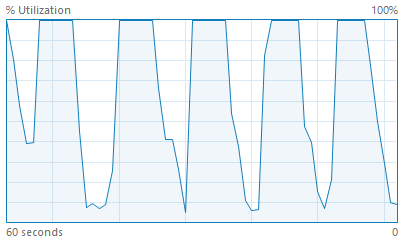
\includegraphics[scale=0.5]{images/cpu_original.png}
\end{center}
The graph looks like a chainsaw, which is a sign that the code is bottle-necked on a single thread.
This is no surprise, since the {\texttt{outputStream} } is written in a sequential fashion.
On top of that, for every row there has to be a mutex check whenever a synchronized block of code is invoked.
Since there is a large number of rows, all these checks will add up and produce a significant slowdown of the overall writing process.

The technique that should have been used in this context involves using a single byte array.
Instead of creating and storing individual string representations of all the {\texttt{SamAlignment} } objects, and writing them one by one to disk, we add progressively information into the buffer.
Only when the buffer becomes full, we write its content on disk.
Obviously, all these steps will be performed in a single thread, but the bottleneck will be less obvious.
The class implementing the byte array is called {\texttt{StreamByteWriter} }.
\begin{verbatim}
StreamByteWriter streamByteWriter 
  = new StreamByteWriter(output);
for (SamAlignment aln: alignments) {
  aln.formatBuffer(streamByteWriter);
}
\end{verbatim}
Even if we are using now a single core for all the writing, the necessary time for creating the output file was reduced by half.
The following graph shows the CPU utilization for this approach:
\begin{center}
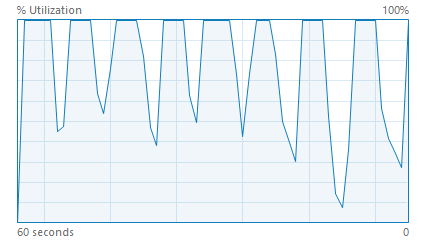
\includegraphics[scale=0.5]{images/cpu_optimized.png}
\end{center}

Here is the execution profile when the Original algorithm has plenty of memory and the "Chainsaw" in execution is in fact that we ran for 50 times the algorithm, and every time the CPU jumps from original 12 core usage when reading to back to 1 Core used and back.
This happens only when executing on "big machines" (when the RAM available is much more than the live set, like 3-4 times at least the size)
\begin{center}
	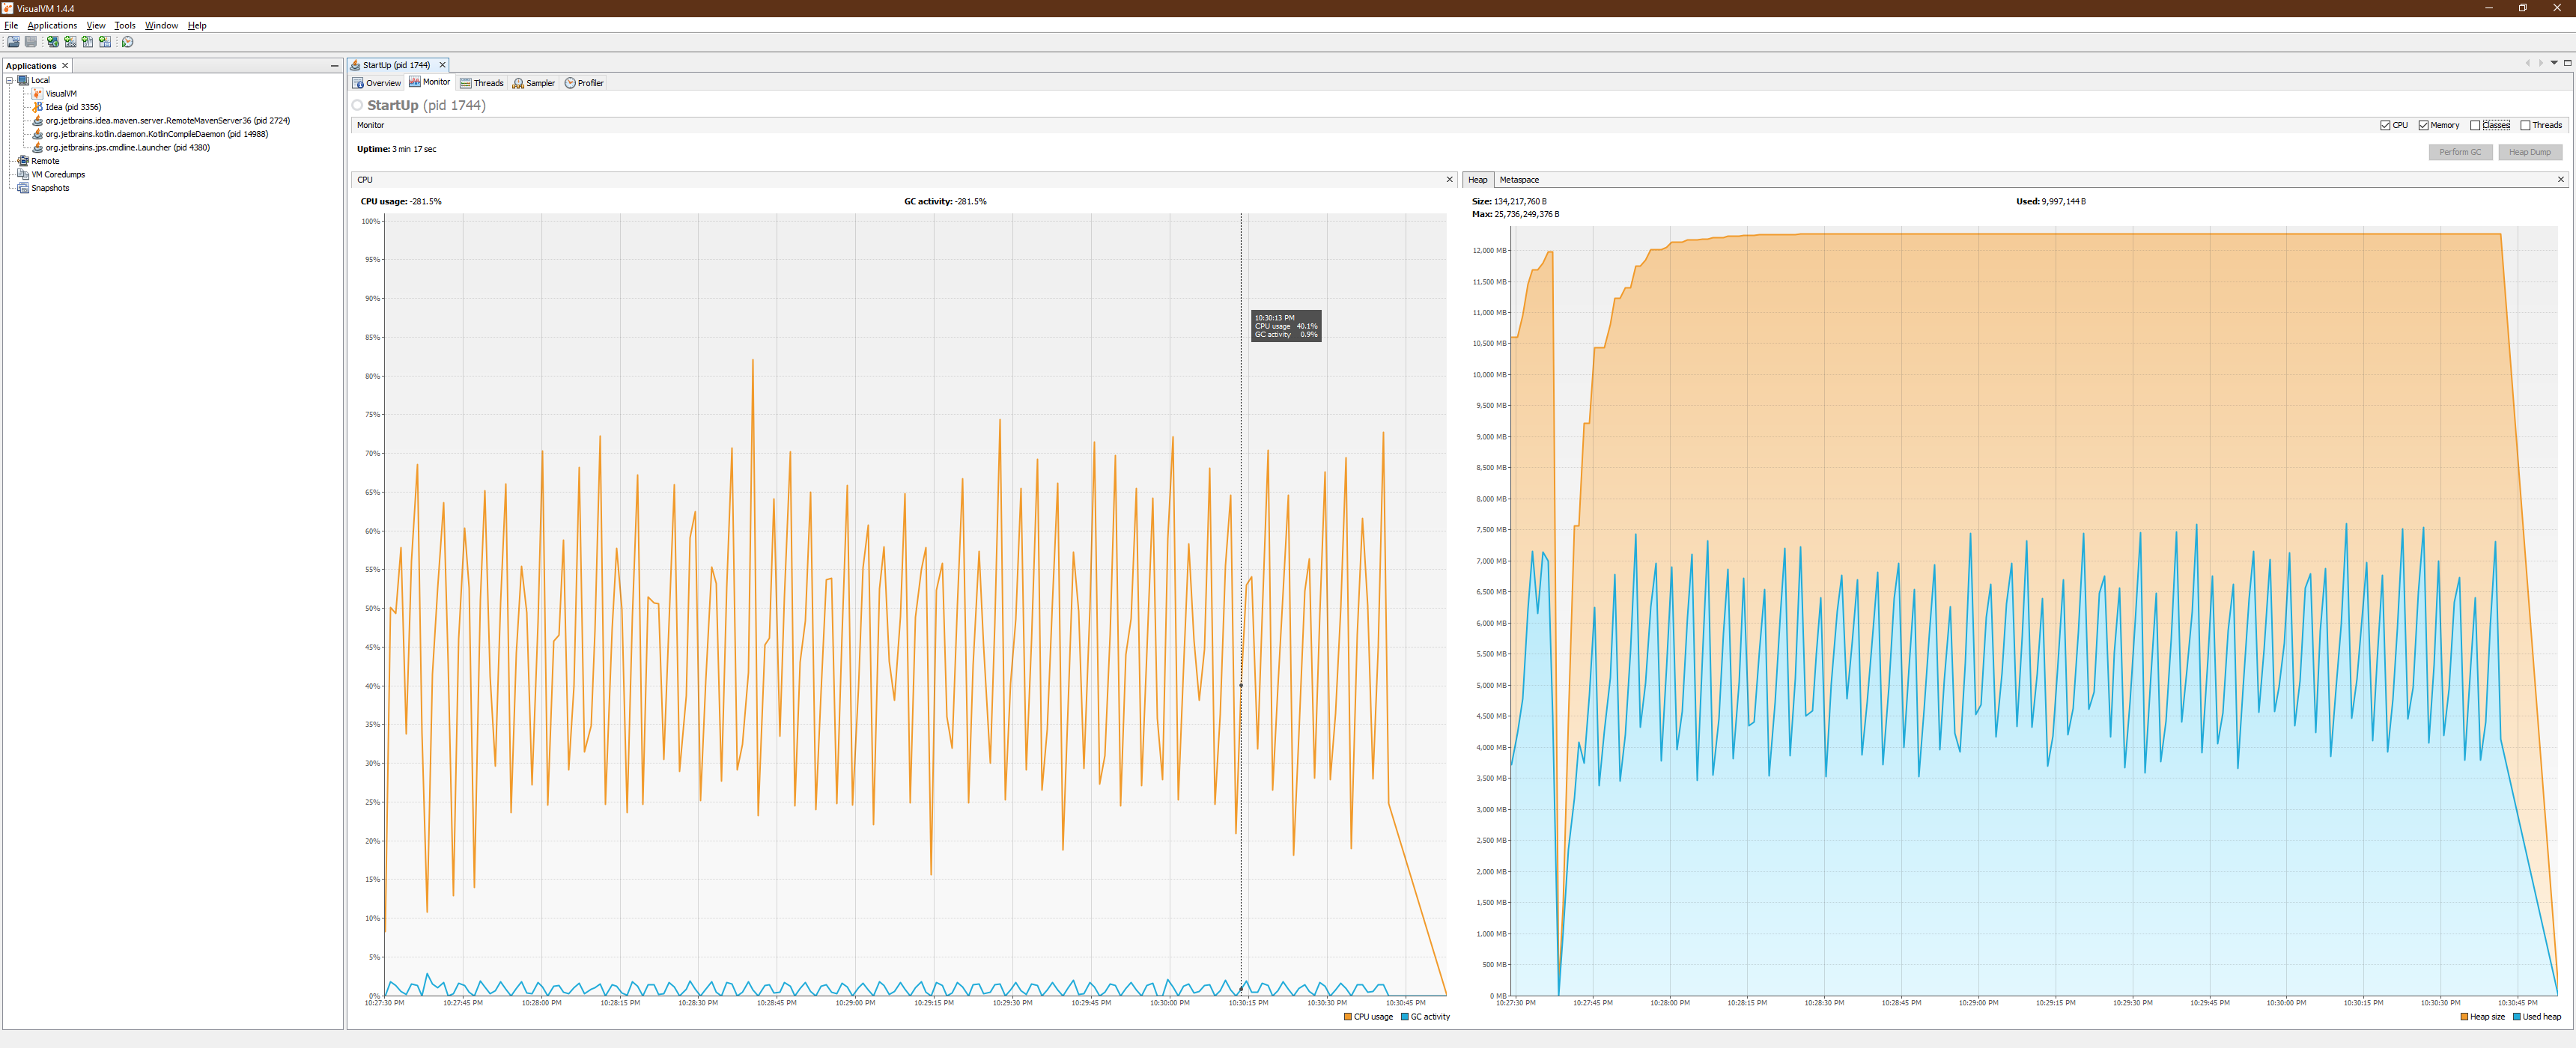
\includegraphics[scale=0.065]{images/Visual_VM_Small_file_Original_execution_profile.png}
\end{center}





\subsection{\uppercase{Chunking-Batching and Extracting Parallelism}}\label{subsec:uppercase10}
%Batch processing is the grouping of similar tasks that require similar resources in order to streamline their completion.
%Chunking is the grouping together of information into ideally sized pieces so they can be used effectively to produce the outcome you want without stress or shutdown.
In the elPrep original algorithm, a {\texttt{SamAlignment} } object is created for each row in the input file.
In order to extract parallelism, there is an explicit {\texttt{.parallel} ()} call, a construct that would create a task for each row that must be processed.
These tasks are queued and executed in a concurrent fashion using threads created transparently by the Java Streams Framework.
\begin{verbatim}
var alnStream = inputStream.parallel()
  .map((s) -> new SamAlignment(s));
\end{verbatim}
In the column-based model, described in section~\ref{model:column}, there is a single {\texttt{SamBatch} } instance storing all the data.
Because we perform data compaction, the {\textit{read} } operation must take into account the dependencies between rows.
Just like in the case of removing duplicates, in order to process a new row we have to inspect the values of the previously read rows.
This means that the reading process cannot be fully parallel per-row.
%(excluding we will use a synchronize/OS Mutex or alike/or a synchronized queue).
%$Even more important, if we would rely on mutexes, the code complexity will be very high and especially debugging this code.
In order to obtain a better performance than reading using a single thread, we propose a technique that splits the {\texttt{SamBatch} } structure in several "chunks".
Instead of having a single large object, we will represent the data using an array of smaller {\texttt{SamBatch} } objects.
A sketch of our {\textit{Compact} } algorithm is described by the following pseudo code:

\begin{verbatim}
int chunkSize = 20000;
int nbOfThreads = cpuCoreCount * 4;
var samBatches = new ArrayList<SamBatch>();
while (!endOfFile) {
  var rowsRead = parallelReadRows(
    batchSize, nbOfThreads);
  parallelTransformRowsIntoBatches(
    samBatches, rowsRead);
}
\end{verbatim}

The {\texttt{readRows} } method reads $chunkSize * nbOfThreads$ rows out of the SAM file for the next processing step.
The actual reading is done using an appropriate number of threads (based on the CPU configuration), each thread reading sequentially a fixed number of rows, calculated taking into account the nature of the information being encoded.
%Even as we want to extract parallelism, this code will likely be almost limited of the speed of the data device (because hard disk are very quick in sequential reads, not as quick on random access).
Having the data split into chunks, we can process in parallel the mapping between the associated text and the {\texttt{SamBatch} } data structure, where we perform data compaction and deduplication.
The techinque of grouping similar tasks requiring the same resources in order to streamline their completion is called {\textit{batching} }.

%Even if we execute in parallel all these steps List<byte[]> -> SamBatch step, there are few advantages:
In our case, the advantages of the chunking-batching approach are multiple:
\begin{itemize}
\item Transforming data, deduplicating and DNA encoding are all executed in a single-threaded manner, which is much easier to debug and understand than a multithreaded equivalent.

\item Since a {\texttt{DeduplicatedDictionary} } will now have less than $20000$ unique strings, the values needed to encode the strings could be represented on $2$ bytes, instead of $4$.
Similarly, we can reduce the tag size from $4$ to $2$ bytes.
%For safety, because technically tags may not always repeat, we used "unsigned short" (meaning "char" type) to better safe around overflowing (which we noticed it happens if user will chose a 30K size SamBatch)

\item After the algorithm is fully executed,  we will have instead of $2.1$ million {\texttt{SamAlignment} } objects, about $105$ {\texttt{SamBatch} } instances, each of them having around $4$ orders of magnitude less objects overall.
This translates into $2$ orders of magnitude less objects.
% yet it has the benefit of memory compaction, low cost on GC and so on

\item When creating the output file, the {\texttt{SamBatch} } array could be processed in parallel, with no blocking except the actual operation of writing to disk.
\end{itemize}

We have seen that the column-based model saves memory at the expense of the running time.
This optimization, however, reduces the overall execution time of the read operation, which is now on par with the original implementation.

When it comes to writing, compared to our {\texttt{StreamByteWriter} } class, which is anyway much faster than the original implementation, the execution time is drastically reduced from $28$ seconds (for the $12$ GB BAM file) to $12$ seconds.
Preparing the strings that are to be written in the file can be done in almost perfect parallelism, using the available cores.
The only limitation remains the speed of the output device, which can vary depending on its type: in memory virtual partition, SSD, HD, etc.
%Even formatting of code is written in almost perfect parallelism (so we talk about 2-3 seconds of fully using the all 12 cores to create formatted buffers to be written, at the end, we are waiting for OS to write the data). 
%To ignore the IO component completely, we used on Windows an "in memory virtual partition".
%Even this could be a limitation of the hardware/OS, we can estimate that IO will be limited eventually on the speed of device or of the Java API to write to disk. 
%The compact algorithm ran against the 5.6 GB SAM file, it can format and write it on a RAM disk in speeds of 500 MB/s, when Java does the in-memory formatting of output in 1 fifth of that, so at a rate of 2500 MB/s (using 12 cores/24 threads though, around).
	
In order to make sure there are no dead times when using the external device, 
we have also implemented the {\textit{async/await} } pattern.
This allows the program to perform in advance reading operations, using a dedicated thread, while waiting for the data processing threads to complete their execution.
This new algorithm, called {\textit{Compact/Par} }, offers a small improvement in the running time, as we will see in the next section, but with the disadvantage of a significant increase in code complexity.
%However, the increase in code complexity makes this optimization hardly worthy of taking it into consideration.
%We added a parallel reader, and this parallel reader increases the complexity of the code, it looks that the improvement is note worthy: on 12c machine/8 GB BAM/SSD the saving of time is from 140 seconds to 131 seconds. On a spinning disk we have from 215 seconds to 195 seconds. On the 4c laptop when processing 1.2 G BAM file, the times improve from 37.43 seconds to 34.1 seconds.
%on 12c machine/8 GB BAM/SSD the saving of time is from 140 seconds to 131 seconds. On a spinning disk we have from 215 seconds to 195 seconds. On the 4c laptop when processing 1.2 G BAM file, the times improve from 37.43 seconds to 34.1 seconds.

%* we can isolate even more a compact version of algorithm (named "Compact parallel") that as it compacts data, it also does prefetching for IO (it reads in a background task the next block that will be needed to be compacted on the next operation),
%and the wins are visible on slow disk, but even using a RAM disk, the algorithm goes even faster (33.38 sec per iteration).






\section{\uppercase{Experimental Results}}\label{sec:uppercase2}

\subsection{\uppercase{Overview}} \label{subsec:uppercase6}

We have created five implementations that address the most expensive parts of the elPrep algorithm, which are reading,  writing and storing all data in the memory. 
Except for the original version, which was taken from elPrep public repository, all other algorithm implementations contain various types of optimization that are meant to improve runtime performance and to lower the memory usage, especially on large files where GC becomes a limiting factor. 
We recap the names of the algorithms as they are used in the following sections:
\begin{itemize}
\item {\it Original}, the original algorithm described in \cite{costanza:2019};

\item {\it PresizedBuffers} reduces the number of memory allocations by carefully constructing the data structures that hold the data to be written, taking into consideration the specific size of the file rows;
%on writing the expected size of the row, eliminating many allocations and especially if the machine's heap reaches the limits of the machine can give a huge speedup. (75 seconds)

\item {\it StreamByteArray} transforms string into bytes and writes them directly into an \texttt{OutputStream}, reducing to almost zero the number of memory allocations related to writing.
%It was achieved without reducing debuggability (meaning that if suspending execution to look for a bug, toString method displays the same relevant data)

\item {\it Compact} employs a more elaborate column-based model for storing the data set in a "compact" form, instead of the simple row-based approach used in the previous two algorithms; this reduces drastically the memory usage at the expense of running time.
%* isolating the slow parts of the original algorithm as being memory heavy and IO heavy (Read-write) we can achieve a comparable performance on read/write, even there is a computational cost on every element, with an observed 4 times less live-memory (34.5 seconds)

\item {\it Compact/Par} represents a modified variant of the {\it Compact} algorithm aimed at reducing to a minimum the dead times regarding I/O operations.

\end{itemize}


The computer we have used in order to perform the experiments is a Ryzen 9-3900X, having 12 cores and using 48 GB of RAM\@.
Since we didn't have access to the hardware necessary to run all the tests in memory, as the original paper, we have used the smaller SAM files and ran the same processing repeatedly in order to obtain an accurate result of the running time.
For example, running $10$ times the algorithm on the smallest input SAM file, which is approximately $700$ MB, will produce a total running time of around $70$ seconds. 
Running the algorithm repeatedly will trigger the garbage collector and this will be the cause of variations in the collected results, ranging from around $2$ to $3$ seconds, when reading the smallest file, and $3$ to $4$ seconds for writing.

Before executing the timed invocations, we have {\textit{warmed-up} } the JVM\@.
This is usually achieved by simply running a couple of times an initial test (not timed) that uses all the classes involved in the algorithm.
Such a warm-up is necessary because Java is using a lazy class loading mechanism and just-in-time compilation.
After this step, all important classes are stored into the JVM cache (native code), making them available at runtime with no additional penalty.

The original elPrep benchmarks have been performed on a Supermicro SuperServer 1029U-TR4T node with two
Intel Xeon Gold 6126 processors consisting of 12 processor cores each, clocked at 2.6 GHz, with 384 GB RAM~\cite{costanza:2019}.
The authors claim to do the processing of the 8 GB BAM file in 6 min:54sec to 7 min:31sec and memory usage is $330-340$ GB\@.

As we didn't have access to such a performing machine, we did most of testing with the smallest file, the $144$ MB BAM file ($673.3$ MB SAM file). For the $8$ GB BAM file ($27.18$ GB SAM) our results will show only the {\it Compact} algorithm but we will make some inferences over the scaling of the original algorithm across file sizes and cores.

Since the elPrep algorithm is designed to run everything in memory, we tuned the JVM heap size (using the \texttt{-Xmx} flag) to the maximum value allowed by the operating system. 
%Especially as elPrep algorithm was using a lot of memory compared to Compact algorithms, we tuned the JVM heap size (using -Xmx flag) to maximum value that the OS would run everything in memory,
%which makes in fact numbers to be a bit better than using just the defaults.
%Without it, values like 123 seconds for original algorithm would degrade into either around 200 seconds mark for runtime or Out-of-memory errors.

In order to analyze the performance of read/write operations, we made sure that no background OS services are running during our tests, by manually stopping them.
%For all algorithms we did use the fastest disk possible (like we were choosing an SSD to read, and if possible, we would be using either RAM or fastest spinning disk).
%And as disk access is sometimes affected by antivirus service in Windows (and as we tested on a regular Windows 10 machine) or background services like Dropbox, OneDrive, etc all services that could be noticed would be manually stopped, and made sure that
%there is no other service running and affecting the numbers (like Windows Updates).
%To try to make sure of no extra factors were affecting performance, Windows Task Manager was running in the background, but it was not found to affect the performance of the tests,
%especially on the 12c machine.




\subsection{\uppercase{Runtime performance}}\label{subsec:uppercase9}

The following table shows a brief comparison of the running times obtained by our algorithms, in three configurations: $144$ MB file using $4$ cores and $12$ cores, and $1.2$ GB file using $12$ cores. 
%The time is expressed in seconds.

\begin{small}
\par
\begin{center}
\textbf{Running time per algorithm in seconds} \\
\begin{tabular}{|C{2cm}|C{1.2cm}|C{1.2cm}|C{1.2cm}|}
\hline
						& 144 MB (4c)	& 144 MB (12c)		& 1.2 GB (12c)	\\ \hline
Original				& 9.13 			& 3.938 			& 123.91 		\\ \hline
PresizedBuffers			& 8.98 			& 4.19 				& 75.1 			\\ \hline
StreamByteArray			& 8.09 			& 3.43 				& 64.62 		\\ \hline
Compact 				& 5.64 			& 3.4 	 			& 34.5			\\ \hline
Compact/Par 			& 5.42		    & 4.68				& 26.7 			\\ \hline
\end{tabular}
\end{center}
\end{small}

Comparing $4$ cores to $12$ cores, we notice that the original algorithm scales with a factor of $2.3$, {\it PresizedBuffers} by a factor of $2.14$, {\it StreamByteArray} scales by $2.36$ and {\it Compact} would scale by $1.69$. So, at least for the small file, it seems that using larger machines will offer a better performance. It is important to notice that, in its current implementation, the {\it Compact} algorithm has an explicit sequential part that reduces its scalability. We address this issue when presenting proposed ideas for potential improvements.
%Analysis of speedup across machines (4 core vs 12 core):
%Original algorithm scales with a factor of 2.3, presized buffers by a factor of 2.14, StreamByteArray scales by 2.36 and compact would scale by: 1.686, so at least for small files it looks that scaling over large machines will be able to offer a better scaling.
%Also, it is important to notice that the compacting algorithm has an explicit sequential part that reduces scalability, and it may be reduced with proposed ideas of potential improvements.

Considering the file size, the original algorithm uses a lot of memory and, since the JVM has to call more often the Garbage Collector, the cost of GC visibly affects the executing time, affecting its scalability. Our techniques of reducing object allocations presented in {\it PresizedBuffers} and {\it StreamByteArray} algorithms pay off now, their runtime profiles are much better than the original. Since the {\it Compact} algorithm reduces drastically the memory consumption, it is not affected too much by GC and the overall running time is significantly superior. 
So, for an increase in file size $8$ times, the original algorithm would slow down $31.46$ times, the {\it PresizedBuffers} will slow down $17.92$ times, {\it StreamByteArray} will slow down $18.83$ times,
and the {\it Compact} algorithm will have a perfect $8.33$ times slow down.

For the $8$ GB BAM file, we could only execute the {\it Compact} algorithm, as the others would produce an \texttt{OutOfMemoryError}, even when setting the heap size to $42$ GB.
The execution time was around $215$ seconds, so as we are reaching the limits of the machine, for a file that is approximately $5$ times larger, the algorithm slows down by a factor of $12$. When moving the input file to an SSD, which offers a faster I/O, the running time drops to $139.8$ seconds, which means a $10$ times slow down.

%As times will grow for a 8 GB BAM file to around 215 seconds (when setting heap size to be 42G as maximum using -Xmx42G), we can investigate and isolate the sequential I/O cost.
%So as we are reaching the limits of the machine, for a file that is approximately 5 times larger, the algorithm slows down by a factor of 12.
%If moving to a bigger batch size (from 20K to 30K), the algorithm will process the output in 133.15 seconds, but for the sake of comparison, it is possible to conclude that using
%fast I/O can improve the runtime performance so the slow-down is from 12 times to 10 times (from 14.08sec to <140 sec).






\subsection{\uppercase{Memory Usage}}\label{subsec:uppercase8}
To measure the live data set, we have used the standard instrumentation tools of the JVM and
Java VisualVM \cite{visualvm:oracle}, which provides a visual interface for profiling a running application. Using VisualVM, we have analyzed the memory consumption in each scenario and we have estimated the minimum amount of memory that JVM requires in order to load a specific data set.
%To measure the live data set, we use the already existing instrumentation in the JVM and the visual tool
%VisualVM to capture according to different algorithms the different values of memory consumption and it describes the minimum amount of memory that JVM has to have available theoretically to load specific data set.
%To get the values from the following paragraphs, it was clicked on the tab "Monitor", look into "Memory" section and we triggered forcefully a GC after we suspended the algorithm when loading all the model (which is the maximum memory used) and it was all used for reading.

Unlike the original paper, which measures process memory size, we have measured live data size.  This is possible due to VisualVM which offers very precise information regarding the objects consuming the memory.
%and many variables are excluded like: the G1GC (the default GC algorithm in Oracle JDK/OpenJDK) uses background threads to free memory which interact with threads of execution, having a quite random values on runtime.
It is also important to understand that the more live memory is used, the more complex the graph of objects is and the less free memory exists on a particular machine, the GC impact will be higher.
This is because the GC algorithm is triggered when a critical amount of the heap is occupied.
Therefore, the more memory JVM has access to, the more seldom GC will execute.
The default {\it Garbage First Garbage Collector (G1 GC)} is automatically triggered at $45\%$ memory occupancy (this value being configurable using the \texttt{InitiatingHeapOccupancyPercent} parameter). When the heap is arriving at this level, JVM will spawn background threads in order to do the marking phase, and this affects the running time.
Having a larger machine with double memory will trigger the GC at least $2$ times more seldom and
although the number of objects to be removed is the same, the overall time necessary for this operation is improved.

%Live data set would let us avoid some of the noise given that most GC algorithms do have typically a "saw teeth" profile, making hard to say how much memory is really used.


\begin{small}
\begin{center}
\textbf{Memory usage per algorithm in MB} \\
	\begin{tabular}{|c|c|c|}
		\hline			  	& 144 MB file		& 1.2 GB file		\\ \hline
		Original			& 2326 MB			& 32025 MB			\\ \hline
		PreSizedBuffers		& 2326 MB			& 32025 MB			\\ \hline
		StreamByteArray 	& 2275 MB			& 31463 MB			\\ \hline
		Compact/Par			& 606 MB			& 4689 MB			\\ \hline
	\end{tabular}
\end{center}
\end{small}

The peak usage was measured by suspending the program at the moment when the whole file was read.
We notice that for the $1.2$ GB BAM file, the {\it Original} and {\it Presized Buffers} algorithms are using around $32$ GB of memory. In order to offer this amount of memory to JVM we used a machine with $48$ GB of RAM. To further reduce the overhead of GC, $64$ GB would certainly have been better.
%Even the live memory set is showing the peak memory usage (by suspending the program and measuring when the whole file is read), on practical terms all algorithms just before finishing (let's say at 99.9 percent mark of finishing reading), would use a bit more live memory but not too much and it is quite hard (if not impossible) to measure it.

%So for example ElPrep "Original" or "Presized Buffers", would use 32 GB of memory at peak usage (in case of 1.2 GB BAM file), so to process it efficiently, probably a machine with 48 GB (with heap tuning, as we did to get best numbers for elPrep, by using -Xmx flag in JVM) or a machine with 64 GB would suffice.

On a $48$ GB machine, {\it Compact} algorithms can process larger files: the $8$ GB BAM file uses $24283$ MB of live data and the $12$ GB BAM input uses $35 265$ MB.


We also have to note that not all of the used memory represents data related to the input file.
For example, in case of the original elPrep algorithm, as it creates millions of tasks even for the smallest $144$ MB BAM file, Java Streams library will create a queue of objects that will remain in memory very likely until the end. This might add maybe around $100$ MB of memory, as it is quite hard (if not impossible) to measure it.
%Similarly the {\it Compact} algorithms would keep in memory the last set of chunks (a batch) that would be similarly even on a large machine under 100 MB and they will be unused right after the related strings are converted into data.

%For all practical purposes, the numbers here are very precise and they would show the range of the machine that could process that data set.




 
 
\subsection{\uppercase{Calculating performance $\times$ memory}} \label{subsec:uppercase7}
The goal of elPrep was to keep both the running time and the the memory consumption low. The evaluation function was defined as the multiplication of the average elapsed wall-clock time (in hours) with the average maximum memory use (in GB), with lower values (in GBh) being better \cite{costanza:2019}.
We have used the same approach, changing only the measurement units to MB and seconds.

In order to analyze the impact of the hardware to the performance of algorithm, we have performed the tests on two distinct machines: the Ryzem 3900X ($1$2 cores and $48$ GB RAM) and a laptop with $4$ cores and $16$ GB RAM.

The results for the $144$ MB file are presented below (lower bars are better):
\begin{center}
	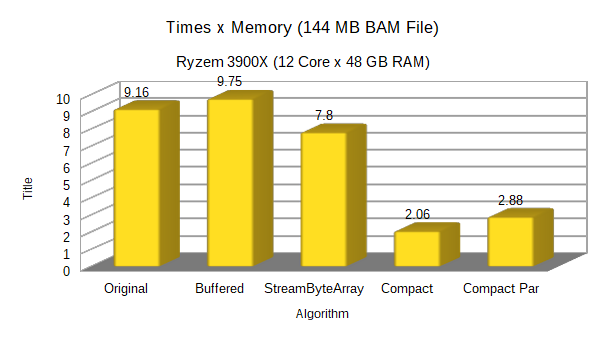
\includegraphics[scale=0.5]{images/times_and_memory_chart_small_144mb_ryzen.png}
\end{center}

As the used memory is quite similar between the original algorithm, {\it PresizedBuffers} and {\it StreamByteArray}, their comparative performance is influenced only by the runtime savings. 
The {\it Compact} algorithms are on par from the point of view of the running time, but since they are using far less memory their performance is much better.
%On very small files, there is a large variation between runtimes as they run just in seconds.

We observe the combination of small size of the file (meaning the algorithm will run just in seconds) and the high core count (12 cores) have a negative impact on the more elaborate algorithm {\it Compact/Par} which has a small slow-down compared to the more simple {\it Compact} implementation.
%has a small slow-down running for 100 times the parallel algorithm which is reflected on the graph:

On the laptop (which has a better SSD), the {\it Compact} algorithm performs even better, since it could not fully exploit the high number of cores in the first test:

\begin{center}
	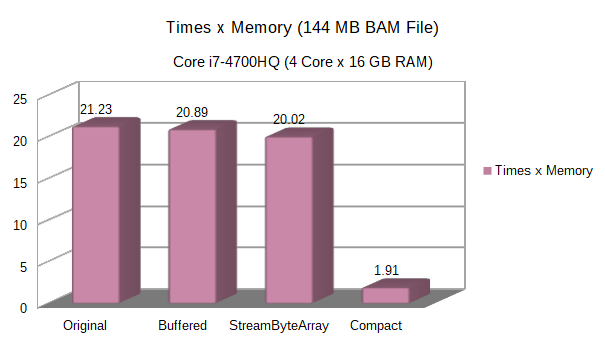
\includegraphics[scale=0.5]{images/times_and_memory_chart_small_144mb_intel.png}
\end{center}


On the medium file ($1.2$ GB BAM) the values are more conclusive from the point of view of scaling the results. The improvements resulting from our optimization techniques are now clearly visible.
%(we have to take into consideration the difference in scale of the machines)

\begin{center}
	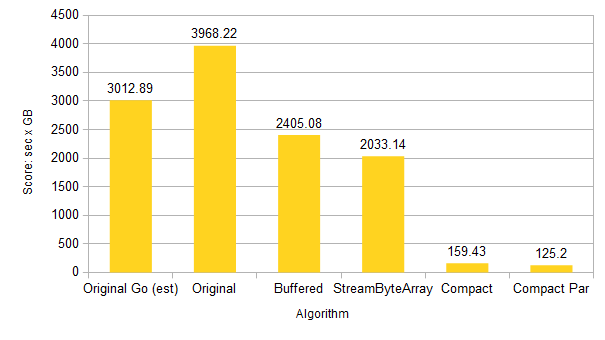
\includegraphics[scale=0.5]{images/times_and_memory_chart.png}
\end{center}

For the larger files, since we could only run the {\it Compact} and {\it Compact/Par} algorithms, and for ElPrep algorithm, we can't make a direct comparison between all algorithms, we can estimate scalability given the files we could run. To not penalize ElPrep, we used StreamByteArray 
version of the algorithm, which should scale better than the original elPrep.  However, tests performed up-to the $8$ GB file showed that they scale as expected, GC does not become a large impediment for both Compact algorithms and the overall performance seems limited only by other hardware components, such as disk drive read/write speeds.
Both Compact algorithms keep a steady pace or processing at around $180$ MB/second (or under 6 seconds to process every 1 GB of BAM). ElPrep (StreamByteArray version) has a sharp loss of speed as GC is triggered more often, processing data at the half of speed when increasing the BAM file size from 0.144 GB to 1.2 GB.
The average values, including both read and write, are presented below:

\begin{center}
	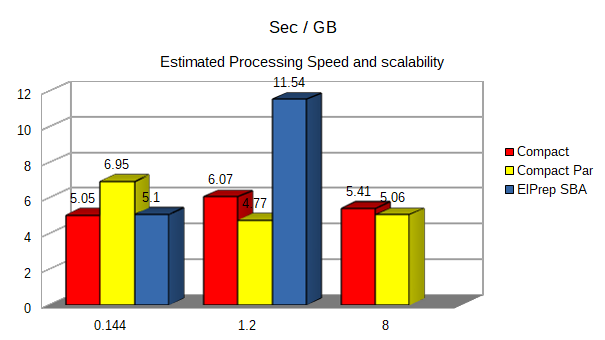
\includegraphics[scale=0.5]{images/seconds_per_gb_ryzen.png}
\end{center}


As for now, these numbers are becoming disk bound (reading speed of the SSD is the limiting component in the system), and it can be speculated how the system would behave if instead of this disk a faster (i.e. NVMe) disk would be used.

Assuming a new disk is used which would remove the disk as the limitation, other component of the system could become the bottleneck. A potential bottleneck could be the rate of Java allocation (also named as "allocation wall", which means that in current
implementations Java could allocate but no faster than a number of MB/sec/core). In the section "Future Work" we propose few techniques that may mitigate or even eliminate these issues.




Given the hardware differences between the machine used by the elPrep authors and ours, there are limits on the testing that could be done with the techniques used by this paper.
Instead of a $384$ GB of memory, dual-CPU server, we have used a machine  with $8$ times less RAM, half of CPU cores, a much slower disk drive (the SSD on the Ryzen machine can barely read at 300 MB/s, while a NVMe SSD can reach $3200$ MB/s) and so on.

Another limitation is that we have ported only the most expensive parts of the algorithm, which are reading,  writing and storing all data in the memory. 
%However, the remaining operations presented in the original paper can be ...
%and we will have a section with possible untested improvements that could be done to get (at least it looks reasonable that) better numbers that are obtained compared with the results that are presented here.












\section{\uppercase{Future work}}\label{sec:uppercase}

\subsection{\uppercase{Scalability of batch reader}}\label{subsec:uppercase5}

Our reader works as described before in two steps:

* it separates initially from the original file into a batch of rows that would be expected to be split later into chunks and batches

* it executes in parallel the compaction step over the separated rows over the all cores

Speeding up the single threaded code by not making allocations

For now, before chunking and batching is done, we split the full byte array read from file into discreet List<byte[]> instances,
but this construct may not be necessary if it is found to be a bottle neck: an alternate approach it would be to store inside the large byte[]
buffer read the end of line character positions, so no splitting is necessary, but it would necessitate some extra code complexity and book keeping.

A similar variation of speeding up the single threaded part is to not do splitting into lines at all, but to read an approximate size in advance that would be around the expected chunk size
and split it after in lines in a multi-threaded way.

\subsection{\uppercase{Testing the code using Value Types}}\label{subsec:uppercase4}

As memory consumption and allocation seem to be large slow-downs inside elPrep and it is having an impact on very large data sets also on the algorithms which we name them Compact,
reducing even by a bit the memory usage and memory compaction.
.Net's Virtual Machine named CLR has a very compact memory implementation of HashMap (System.Generic.Dictionary class) that could be possibly giving even more memory savings.
Similarly, there is an effort named Project Valhalla in JVM that has previews to download that can technically implement a memory compact dictionary that may have the same memory savings.

So just porting to .Net the code may bring less memory usage and maybe some speedups.

\subsection{\uppercase{Doing the algorithms}}\label{subsec:uppercase3}

When implementing the Compact algorithms, it was implemented only the read/write and materialization of the data set stored in SAM/BAM files, as it was a very expensive part of the
elPrep implementation.

Though the data in-memory has to be reordered, filtered, deleted from invalid data, and so on.
These algorithms very likely can be very easily made in parallel (as any chunk is a parallel subset of the entire file), but it isn't both the point of this paper as it focused
only on memory usage and very fast reading/writing.

Some notes can be easily expected:

* some tasks can be integrated into reading before inserting data into SamBatch structures, but it will be at a cost of code complexity,
so a more sensible approach would be to read first, then do algorithms one by one in a parallel fashion
* filtering and deleting data in general will have to include two steps (or a secondary SamBatch which rebuids from the first only with items that pass the condition)
* sorting is possible as the batches are directly indexable, so item with number: 654321 would be on SamBatch index 654 321 / 20 000, and with sub-index inside the batch of 654321 \% 20 000
* another way to do the sorting is to sort inside the batch first by sequences (and sequences are easily sortable as the sorting is done 21 DNA letters at once) inside the batch,
then a merge sort could be done across the SamBatch(es)

\subsection{\uppercase{Conclusions}}\label{subsec:uppercase2}

The presented techniques in this paper show that in algorithms where the task is heavily limited by memory allocation(s), just by reducing reducing the rate of GC trough removing many small allocations, it can improve significantly the runtime performance.
We measured a speedup factor of 2 in large files just by writing sequentially and not allocating anything as we write the bytes ourselves by tuning ElPrep algorithm without changing the semantics.

As elPrep stores a large data-set looking like a large CSV file - and for similar applications that need to store large data sets in memory - techniques of memory compaction, especially tuned per type of column, 
can reduce significantly the memory usage without reducing the performance of  application, compaction time being typically less than calling underlying garbage collection.

If memory compaction is mixed with chunked data and batching the chunks are taken proportional with numbers of physical cores, the algorithm can extract parallelism making the code to be comparable with implementations that extract good parallelism as is elPrep.

Using parallel fetching as the algorithm of memory compaction is happening (algorithm named by us "Compact Par"), it can improve even more the performance for these algorithm (from 159 sec/GB to 125 se/cGB).


\begin{comment}

\subsection*{Original}
As Java GC does use more system memory to speedup allocations, it is important to see how real life memory usage is calculated.

To calculate live memory usage we took VisualVM toolset and we got a memory snapshot just before all writing to disk was done. In this way we know that all data set is processed in memory and no data is discarded.


Here is a screenshot of the original algorithm with a heap dump:
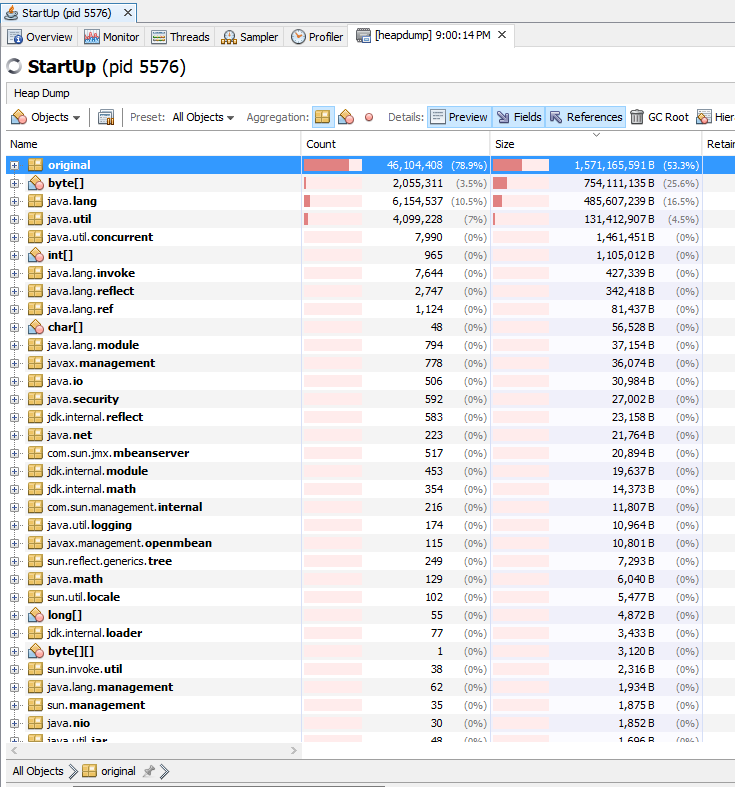
\includegraphics[scale=0.33]{images/VisualVM_Orig_144MB_heap_dump}

The main difference over the "Optimized" algorithm is the 2.5M strings and 78M bytes associated with them

\subsection*{Optimized}

As "Optimized" algorithm is mostly a tuned implementation of Original, but it tries to materialize as little intermediate objects, the heap will look very similar:

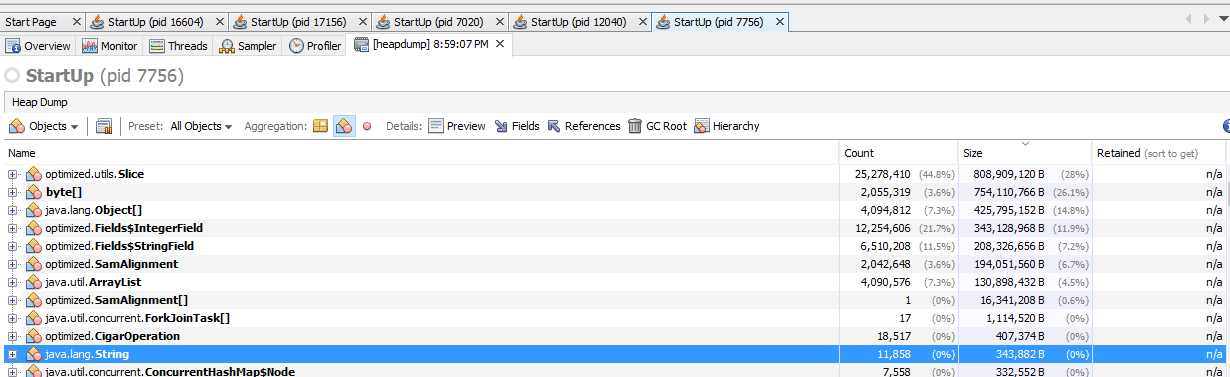
\includegraphics[scale=0.33]{images/VisualVM_Optimized_144MB_heap_dump}

\subsection*{Compact}

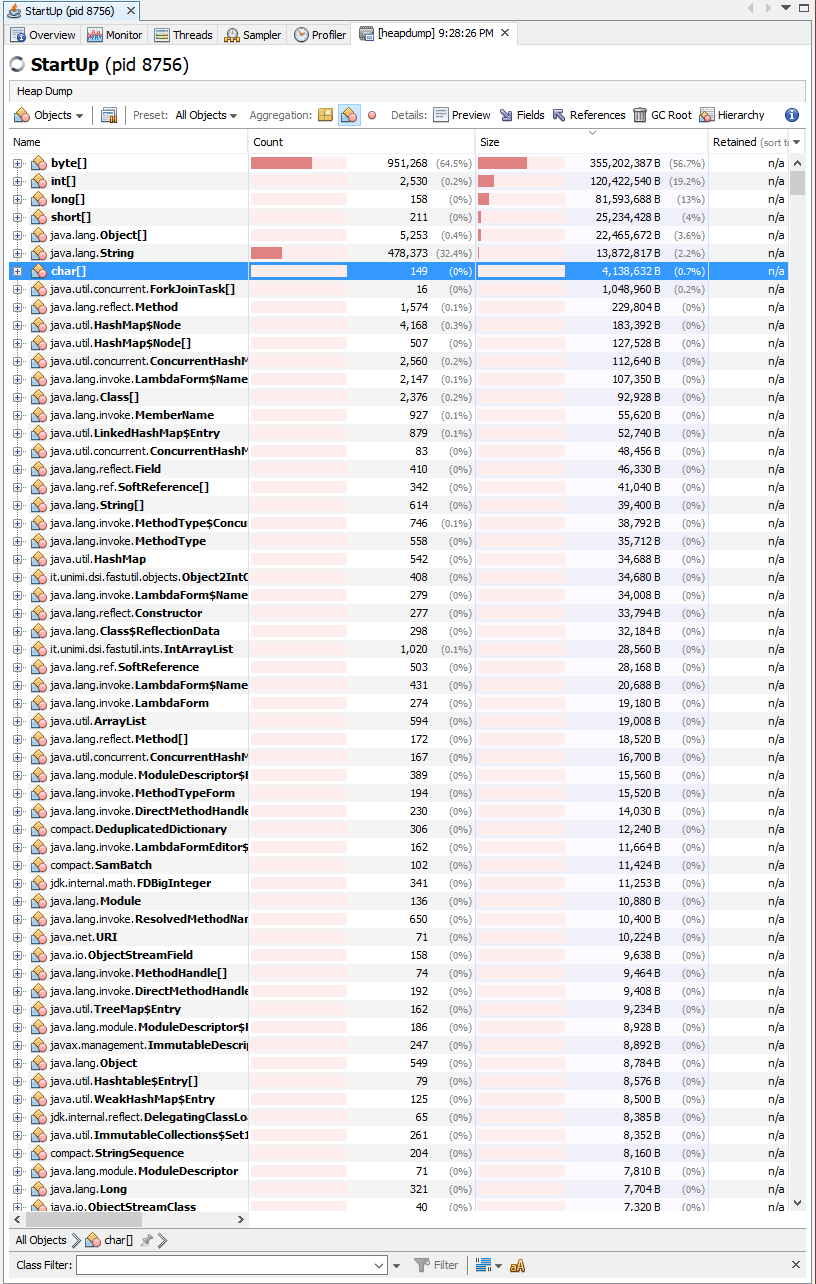
\includegraphics[scale=0.33]{images/VisualVM_Compact_144MB_heap_dump}

What is critical to be observed is simply that the Compact uses for all types that use up-to 1M instances of live data, the full heap dump was only of: 624.066 M Bytes, 
when compared with Original or Optimized implementations that they were floating over 4.5 times more live memory usage (or 3 GB).

\end{comment}


\bibliographystyle{apalike}
{\small
\bibliography{elprep-study}}


\end{document}

